\documentclass[11pt,a4paper]{article}
\usepackage[english,greek]{babel}
\usepackage[utf8]{inputenc}
\usepackage{nimbusserif}
\usepackage[T1]{fontenc}
\usepackage[left=2.00cm, right=2.00cm, top=3.00cm, bottom=2.00cm]{geometry}
\usepackage{amsmath}
\let\myBbbk\Bbbk
\let\Bbbk\relax
\usepackage[amsbb,subscriptcorrection,zswash,mtpcal,mtphrb,mtpfrak]{mtpro2}
\usepackage{graphicx,multicol,multirow,enumitem,tabularx,mathimatika,gensymb,venndiagram,hhline,longtable,tkz-euclide,fontawesome5,eurosym,tcolorbox,wrap-rl}
\tcbuselibrary{skins,theorems,breakable}
\newlist{rlist}{enumerate}{3}
\setlist[rlist]{itemsep=0mm,label=\roman*.}
\newlist{alist}{enumerate}{3}
\setlist[alist]{itemsep=0mm,label=\alph*.}
\newcommand{\lysh}{\textcolor{black}{\textbf{\faCheck\ \ ΛΥΣΗ}}}
\renewcommand{\textstigma}{\textsigma\texttau}
%----------- ΟΡΙΣΜΟΣ------------------
\newcounter{orismos}[section]
\renewcommand{\theorismos}{\thesection.\arabic{orismos}}   
\newcommand{\Orismos}{\refstepcounter{orismos}{\textbf{\textcolor{black}{\kerkissans{Ορισμός\hspace{2mm}\theorismos}}\;:\;}{}}}

\newenvironment{orismos}[1]
{\begin{tcolorbox}[title=\Orismos {\textcolor{black}{\kerkissans{#1}}},breakable,bottomtitle=-1.5mm,
enhanced standard,titlerule=-.2pt,toprule=0pt, rightrule=0pt, bottomrule=0pt,
colback=white,left=2mm,top=1mm,bottom=0mm,
boxrule=0pt,
colframe=white,borderline west={1.5mm}{0pt}{black},leftrule=2mm,sharp corners,coltitle=black]}
{\end{tcolorbox}}

\newcommand{\kerkissans}[1]{{\fontfamily{maksf}\selectfont \textbf{#1}}}

\begin{document}
\begin{center}
{\LARGE \textbf{Τυπολόγιο}}\\
{\Large \textbf{Μαθηματικά Κατεύθυνσης}}
\end{center}
\section{Διανύσματα}
\subsection{Η έννοια του διανύσματος}
\begin{enumerate}
\item Διάνυσμα: Προσανατολισμένο ευθύγραμμο τμήμα:
\begin{center}
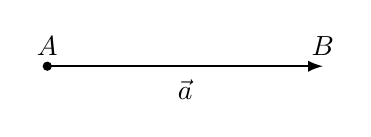
\begin{tikzpicture}
\draw[-latex,line width=.3mm] (0,1) node[anchor=south] (A){$A
$}--(3.5,1) node[anchor=south] (B){$B
$};
\node(a) at (1.75,.7){$ \vec{a} $};
\tkzDrawPoint[size=2.9,fill=black](0,1)
\end{tikzpicture}\qquad $ A $: αρχή\ \ ,\ \ $ B $: πέρας.
\end{center}
\begin{multicols}{2}
\item Ομόρροπα διανύσματα: $ \vec{a}\upuparrows\vec{\beta} $.
\item Αντίρροπα διανύσματα: $ \vec{a}\downuparrows\vec{\beta} $.
\end{multicols}
\item Ίσα διανύσματα: $ \vec{a}=\vec{\beta} $. Έχουν ίσα μέτρα και ίδια κατεύθυνση.
\item Αντίθετα διανύσματα: $ \vec{a}=-\vec{\beta} $. Έχουν ίσα μέτρα και αντίθετες κατευθύνσεις.
\begin{multicols}{2}
\item Γωνία διανυσμάτων: $ \GwniaDianysmatwn{a}{\beta} $.
\item Μέτρο διανύσματος: $ |\vec{a}| $.
\end{multicols}
\end{enumerate}
\subsection{Πρόσθεση διανυσμάτων}
\begin{enumerate}
\begin{multicols}{2}
\item Διαδοχικά διανύσματα:
\vspace{-5mm}
\begin{center}
\begin{tikzpicture}
\Dianysma[color=black]{0,0}{2.7,.5}{E}{Z}
\Dianysma{0,0}{1.5,1}{A}{B}
\Dianysma{1.5,1}{2.7,.5}{C}{D}
\tkzLabelPoint[above](A){$O$}
\tkzLabelPoint[above](B){$A$}
\tkzLabelPoint[right](D){$B$}
\node at (.7,.77){$\vec{a}$};
\node at (2.2,1.04){$\vec{\beta}$};
\node at (1.4,-.05){$\vec{a}+\vec{\beta}$};
\node at (1.5,-.77){$\vec{a}+\vec{\beta}=\overrightarrow{OA}+\overrightarrow{AB}=\overrightarrow{OB}$};
\end{tikzpicture}
\end{center}
\item Κανόνας παραλληλογράμμου:
\vspace{-5mm}
\begin{center}
\begin{tikzpicture}
\Dianysma[color=black]{0,0}{3.4,1.5}{E}{Z}
\Dianysma{0,0}{1,1.5}{A}{B}
\Dianysma{0,0}{2.4,0}{C}{D}
\draw[dashed] (2.4,0)--(3.4,1.5);
\draw[dashed] (1,1.5)--(3.4,1.5);
\tkzLabelPoint[left](A){$O$}
\tkzLabelPoint[above](B){$A$}
\tkzLabelPoint[right](D){$B$}
\tkzLabelPoint[right,yshift=1mm](Z){$M$}
\node at (.2,.77){$\vec{a}$};
\node at (1.2,-.33){$\vec{\beta}$};
\node[rotate=23.8] at (1.4,.9){$\vec{a}+\vec{\beta}$};
\node at (1.5,-.77){$\vec{a}+\vec{\beta}=\overrightarrow{OA}+\overrightarrow{OB}=\overrightarrow{OM}$};
\end{tikzpicture}
\end{center}
\end{multicols}
\item Ιδιότητες πρόσθεσης διανυσμάτων:
\begin{center}
\begin{tabular}{cc|cc}
\hline \rule[-2ex]{0pt}{5.5ex} \textbf{Ιδιότητα} & \textbf{Συνθήκη} & \textbf{Ιδιότητα} & \textbf{Συνθήκη}  \\ 
\hhline{====} \rule[-2ex]{0pt}{5.5ex} Αντιμεταθετική & $ \vec{a}+\vec{\beta}=\vec{\beta}+\vec{a} $ & Ουδέτερο στοιχείο & $ \vec{a}+\vec{0}=\vec{a} $ \\ 
 \rule[-2ex]{0pt}{5.5ex} Προσεταιριστική & $ \vec{a}+\left( \vec{\beta}+\vec{\gamma}\right) =\left( \vec{a}+\vec{\beta}\right) +\vec{\gamma} $ & Αντίθετα διανύσματα & $ \vec{a}+(-\vec{a})=\vec{0} $ \\
\hline 
\end{tabular}
\end{center}
\item Διάνυσμα θέσης:\\
\wrapr{-10mm}{5}{7cm}{-5mm}{\begin{tikzpicture}
\Dianysma{0,0}{.75,1.5}{O}{A}
\Dianysma{0,0}{2.5,1}{O}{B}
\Dianysma{.75,1.5}{2.5,1}{A}{B}
\draw (0.75,1.5) -- (2.5,1);
\tkzLabelPoint[left](O){$O$}
\tkzLabelPoint[above](A){$A$}
\tkzLabelPoint[above,xshift=2mm](B){$B$}
\node at (5,.75){$\overrightarrow{AB}=\overrightarrow{OB}-\overrightarrow{OA}$};
\end{tikzpicture}}{
\begin{itemize}
\item $ \DianysmaBelos{OA},\DianysmaBelos{OB} $ διανυσματικές ακτίνες των $ A,B $
\item $ O $ σημείο αναφοράς.
\end{itemize}}\mbox{}\\\\
\item Μέτρο αθροίσματος διανυσμάτων: $ \left||\vec{a}|-|\vec{\beta}| \right| \leq\left|\vec{a}+\vec{\beta}\right|\leq|\vec{a}|+|\vec{\beta}| $
\end{enumerate}
\subsection{Γινόμενο αριθμού με διάνυσμα}
\begin{enumerate}
\item Γινόμενο αριθμού με διάνυσμα: $ \lambda\cdot\vec{a} $.
\item Γραμμικός συνδυασμός: $ \vec{\delta}=\lambda\cdot\vec{a}+\mu\cdot\vec{\beta} $.
\item Ιδιότητες πολλαπλασιασμού:
\begin{center}
\begin{longtable}{cc}
\hline \rule[-2ex]{0pt}{5.5ex} \textbf{Ιδιότητα} & \textbf{Συνθήκη} \\ 
\hhline{==} \rule[-2ex]{0pt}{5.5ex} Επιμεριστική (ως προς αριθμό) & $ \lambda\left( \vec{a}\pm\vec{\beta}\right)=\lambda\cdot\vec{a}\pm\lambda\cdot\vec{\beta} $ \\ 
\rule[-2ex]{0pt}{5.5ex} Επιμεριστική (ως προς διάνυσμα) & $ \left( \lambda\pm\mu\right)\cdot\vec{a}=\lambda\cdot\vec{a}\pm\mu\cdot\vec{a} $ \\
\rule[-2ex]{0pt}{5.5ex} Προσεταιριστική & $ \lambda\left( \mu\vec{a}\right)=\left( \lambda\cdot\mu\right)\cdot\vec{a} $ \\ 
\rule[-2ex]{0pt}{5.5ex} Μηδενικό γινόμενο & $ \lambda\cdot\vec{a}=\vec{0}\Leftrightarrow \lambda=0 \ \textrm{ή}\ \vec{a}=\vec{0} $ \\ 
\rule[-2ex]{0pt}{5.5ex} Πρόσημο γινομένου & $ \left( -\lambda\cdot\vec{a}\right)=(-\lambda)\cdot\vec{a}=-\left( \lambda\cdot\vec{a}\right)  $ \\ 
\rule[-2ex]{0pt}{5.5ex} Νόμος διαγραφής (ως προς διάνυσμα) & Αν $ \lambda\cdot\vec{a}=\mu\cdot\vec{a} $ και $ \vec{a}\neq0 $ τότε $ \lambda=\mu $ \\ 
\rule[-2ex]{0pt}{5.5ex} Νόμος διαγραφής (ως προς αριθμό) & Αν $ \lambda\cdot\vec{a}=\lambda\cdot\vec{\beta} $ και $ \lambda\neq0 $ τότε $ \vec{a}=\vec{\beta} $\\ 
\hline 
\end{longtable}
\end{center}
\vspace{-5mm}
\item Συνθήκη παραλληλίας διανυσμάτων: $ \vec{a}\parallel\vec{\beta}\Leftrightarrow \vec{a}=\lambda\cdot\vec{\beta}\ ,\ \lambda\in\mathbb{R} $.
\item Διανυσματική ακτίνα μέσου διανύσματος: $ \overrightarrow{OM}=\dfrac{\overrightarrow{OA}+\overrightarrow{OB}}{2} $
\end{enumerate}
\subsection{Συντεταγμένες διανύσματος}
\begin{enumerate}
\begin{multicols}{2}
\item Συντεταγμένες διανύσματος: $ \vec{a}=(x,y) $.
\item Ίσα διανύσματα $ \vec{a}=\vec{\beta}\Leftrightarrow x_1=x_1\ \ \textrm{και}\ \ y_1=y_2 $.
\end{multicols}
\item Μηδενικά διανύσματα : $ \vec{a}=0\Leftrightarrow x=0 $ και $ y=0 $\ \ ,\ \ 
$ \vec{a}\neq0\Leftrightarrow x\neq0 $ ή $ y\neq0 $
\item Οριζόντια και κατακόρυφα διανύσματα :
$ \vec{a}\parallel x'x\Leftrightarrow y=0 $ και $ \vec{a}\parallel y'y\Leftrightarrow x=0 $
\item Πράξεις μεταξύ διανυσμάτων:
\begin{center}
\begin{tabular}{cc}
\hline \rule[-2ex]{0pt}{5.5ex} \textbf{Πράξη} & \textbf{Συντεταγμένες} \\ 
\hhline{==} \rule[-2ex]{0pt}{5.5ex} Άθροισμα & $ \vec{a}+\vec{\beta}=(x_1,y_1)+(x_2,y_2)=(x_1+x_2,y_1+y_2) $ \\ 
 \rule[-2ex]{0pt}{5.5ex} Πολλαπλασιασμός & $ \lambda\cdot\vec{a}=\lambda(x_1,y_1)=(\lambda x_1,\lambda y_1) $ \\ 
 \rule[-2ex]{0pt}{5.5ex} Γραμμικός συνδυασμός & $ \lambda\vec{a}+\mu\vec{\beta}=\lambda(x_1,y_1)+\mu(x_2,y_2)=(\lambda x_1+\mu x_2,\lambda y_1+\mu y_2) $ \\ 
\hline 
\end{tabular}
\end{center}
\item Συντεταγμένες μέσου διανύσματος: $ x_{M}=\frac{x_{A}+x_{B}}{2}\quad,\quad y_{M}=\frac{y_{A}+y_{B}}{2} $.
\item Συντεταγμένες διανύσματος με γνωστά άκρα: $ \overrightarrow{AB}=\left(x_2-x_1,y_2-y_1 \right) $.
\item Συντελεστής διεύθυνσης διανύσματος $ \vec{a}=(x,y) $:\[  \lambda=\dfrac{y}{x}=\ef{\omega} \text{ όπου } \omega \text{ είναι η γωνία του } \vec{a} \text{ με τον } x'x \]
\item Συνθήκες παραλληλίας διανυσμάτων:
\begin{rlist}
\item Οι συντελεστές διεύθυνσης των διανυσμάτων είναι ίσοι : $ \vec{a}\parallel\vec{\beta}\Leftrightarrow \lambda_1=\lambda_2 $.
\item Η ορίζουσα $ \det{(\vec{a},\vec{\beta})} $ των συντεταγμένων των διανυσμάτων ισούται με το $ 0 $.
\[  \vec{a}\parallel\vec{\beta}\Leftrightarrow \det{(\vec{a},\vec{\beta})}=\begin{vmatrix}
x_1 & y_1\\x_2 & y_2
\end{vmatrix}=0 \]
\end{rlist}
\item Μέτρο διανύσματος $ \vec{a}=(x,y) $:\ $ |\vec{a}|=\sqrt{x^2+y^2} $.
\item Μέτρο διανύσματος με γνωστά άκρα: $ \overrightarrow{AB}=\sqrt{(x_2-x_1)^2+(y_2-y_1)^2} $.
\end{enumerate}
\subsection{Εσωτερικό γινόμενο}
\begin{enumerate}
\item Εσωτερικό γινόμενο: $ \vec{a}\cdot\vec{\beta}=|\vec{a}||\vec{\beta}|\syn{\varphi} $.
\item Ιδιότητες εσωτερικού γινομένου:
\begin{center}
\begin{longtable}{cc|cc}
\hline \rule[-2ex]{0pt}{5.5ex} \textbf{Ιδιότητα} & \textbf{Συνθήκη} & \textbf{Ιδιότητα} & \textbf{Συνθήκη} \\ 
\hhline{====}  \rule[-2ex]{0pt}{5.5ex} \textbf{Κάθετα διανύσματα} & Αν $ \vec{a}\bot\vec{\beta}\Leftrightarrow \vec{a}\cdot\vec{\beta}=0 $ & \textbf{Αντιμεταθετική} & $ \vec{a}\cdot\vec{\beta}=\vec{\beta}\cdot\vec{a} $ \\ 
 \rule[-2ex]{0pt}{5.5ex} \textbf{Ομόρροπα } & $ \vec{a}\upuparrows\vec{\beta}\Leftrightarrow \vec{a}\cdot\vec{\beta}=|\vec{a}|\cdot|\vec{\beta}| $ & \textbf{Προσεταιριστική} & $ \mu(\vec{a}\cdot\vec{\beta})=(\mu\vec{\beta})\cdot\vec{a} $ \\ 
 \rule[-2ex]{0pt}{5.5ex} \textbf{Αντίρροπα} & $ \vec{a}\updownarrows\vec{\beta}\Leftrightarrow \vec{a}\cdot\vec{\beta}=-|\vec{a}|\cdot|\vec{\beta}| $ & \textbf{Επιμεριστική} & $ \vec{a}\cdot\left( \vec{\beta}+\vec{\gamma}\right) =\vec{a}\cdot\vec{\beta}+\vec{a}\cdot\vec{\gamma} $ \\ 
 \rule[-2ex]{0pt}{5.5ex} \textbf{Τετράγωνο διανύσματος} & $ \vec{a}^2=|\vec{a}|^2 $ & & \\ 
\hline 
\end{longtable} 
\end{center}
\vspace{-7mm}
\item Συνθήκη καθετότητας διανυσμάτων: $ \lambda_{\vec{a}}\cdot\lambda_{\vec{\beta}}=-1 $.
\item Αναλυτική έκφραση εσωτερικού γινομένου διανυσμάτων: $ \vec{a}\cdot\vec{\beta}=x_1x_2+y_1y_2 $.
\item Συνημίτονο γωνίας διανυσμάτων: $ \syn{(\widehat{\vec{a},\vec{\beta}})}=\dfrac{\vec{a}\cdot\vec{\beta}}{|\vec{a}|\cdot|\vec{\beta}|}=\dfrac{x_1x_2+y_1y_2}{\sqrt{x_1^2+y_1^2}\cdot\sqrt{x_2^2+y_2^2}} $
\end{enumerate}
\newpage
\section{Ευθεία}
\subsection{Η ευθεία \bmath{$ y=ax+\beta $}}
\begin{enumerate}
\item Απλή μορφή εξίσωσης ευθείας: $ y=ax+\beta $.
\item Συντελεστής διεύθυνσης ευθείας: 
\begin{itemize}
\item $ \lambda=\ef{\omega}=\dfrac{y}{x} $ όπου $ \omega=x\hat{O}M $ με $ M(x,y) $ σημείο της ευθείας.
\item $ \lambda=\dfrac{y_2-y_1}{x_2-x_1} $ όπου $ A(x_1,y_1) $ και $ B(x_2,y_2) $ είναι δύο σημεία της ευθείας.
\end{itemize}
\item Εξίσωση ευθείας: $ y-y_0=\lambda(x-x_0) $
\begin{itemize}
\item Εξίσωση οριζόντιας ευθείας $ y=y_0 $.
\item Εξίσωση κατακόρυφης ευθείας $ x=x_0 $.
\end{itemize}
\item Συνθήκες παραλληλίας και καθετότητας ευθειών: Αν $ \varepsilon_1\parallel\DianysmaBelos{\delta_1} $ και $ \varepsilon_2\parallel\DianysmaBelos{\delta_2} $ τότε
\begin{itemize}
\item $ \varepsilon_1\parallel\varepsilon_2\Leftrightarrow\lambda_1=\lambda_2 $\ \  ή\ \  $ \det{\left(\DianysmaBelos{\delta_1},\DianysmaBelos{\delta_2}\right)}=0 $
\item $ \varepsilon_1\bot\varepsilon_2\Leftrightarrow\lambda_1\cdot\lambda_2=-1 $\ \ ή\ \ $ \DianysmaBelos{\delta_1}\cdot\DianysmaBelos{\delta_2}=0 $.
\end{itemize}
\end{enumerate}
\subsection{Γενική μορφή εξίσωσης ευθείας}
\begin{enumerate}
\item Γενική μορφή εξίσωσης ευθείας: $ Ax+By+\varGamma=0 $ με $ A\neq0 $ ή $ B\neq0 $.
\item Συντελεστής διεύθυνσης: $ \lambda=-\dfrac{A}{B} $.
\item Παράλληλο διάνυσμα: $ \varepsilon\parallel\DianysmaBelos{\delta}=(B,-A) $\ \ ή\ \ $ \DianysmaBelos{\delta}=(-B,A) $.
\item Κάθετο διάνυσμα: $ \varepsilon\bot\DianysmaBelos{n}=(A,B) $\ \ ή\ \ $ \DianysmaBelos{n}=(-A,-B) $.
\item Γωνία $ \varphi $ δύο ευθειών $ \varepsilon_1 $ και $ \varepsilon_2 $: $ \syn{\varphi}=\syn{GwniaDianysmatwn{\delta_{1}}{\delta_{2}}}=\dfrac{\DianysmaBelos{\delta}_{1} \cdot \DianysmaBelos{\delta}_{2}}{\left|\DianysmaBelos{\delta}_{1}\right|\left|\DianysmaBelos{\delta}_{2}\right|}$ όπου $ \varepsilon_1\parallel\DianysmaBelos{\delta_1} $ και $ \varepsilon_2\parallel\DianysmaBelos{\delta_2} $.
\end{enumerate}
\subsection{Απόσταση σημείου από ευθεία}
\begin{enumerate}
\item Απόσταση σημείου από ευθεία: $ d(A,\varepsilon)=\dfrac{|Ax_0+By_0+\varGamma|}{\sqrt{A^2+B^2}} $.
\item Απόσταση παράλληλων ευθειών $ \varepsilon_1:y=\lambda x+\beta_1 $ και $ \varepsilon_2:y=\lambda x+\beta_2 $. 
\[ d(\varepsilon_1,\varepsilon_2)=\dfrac{|\beta_1-\beta_2|}{\sqrt{\lambda^2+1}} \]
\item Εμβαδόν ενός τριγώνου $ AB\varGamma $ με κορυφές $ A(x_1,y_1),B(x_2,y_2) $ και $ \varGamma(x_3,y_3) $:
\[ (AB\varGamma)=\frac{1}{2}\left|\det{(\overrightarrow{AB},\overrightarrow{A\varGamma})} \right|=\frac{1}{2}\left|\det{(\overrightarrow{AB},\overrightarrow{B\varGamma})} \right|=\frac{1}{2}\left|\det{(\overrightarrow{B\varGamma},\overrightarrow{A\varGamma})} \right| \]
\end{enumerate}
\newpage
\section{Κωνικές τομές}
\subsection{Κύκλος}
\begin{enumerate}
\item Εξίσωση με κέντρο $ O(0,0) $:\quad $ x^2+y^2=\rho^2 $.
\item Εξίσωση με κέντρο $ K(x_0,y_0) $:\quad $ (x-x_0)^2+(y-y_0)^2=\rho^2 $.
\item Εξίσωση εφαπτομένης στο $ A(x_1,y_1) $ του κύκλου με κέντρο $ O(0,0) $:\quad $ xx_1+yy_1=\rho^2 $.
\item Γενική εξίσωση κύκλου:\quad $ x^2+y^2+Ax+By+\varGamma=0 $
\begin{rlist}
\item Αν $ A^2+B^2-4\varGamma>0 $ τότε η εξίσωση παριστάνει κύκλο με κέντρο $ K\left(-\frac{A}{2},-\frac{B}{2} \right) $ και ακτίνα $ \rho=\frac{\sqrt{A^2+B^2-4\varGamma}}{2} $.
\item Αν $ A^2+B^2-4\varGamma=0 $ τότε η εξίσωση παριστάνει το σημείο $ K\left(-\frac{A}{2},-\frac{B}{2} \right) $.
\item Αν $ A^2+B^2-4\varGamma<0 $ τότε η εξίσωση δεν αντιστοιχεί σε σχήμα.
\end{rlist}
\end{enumerate}
\subsection{Παραβολή}
\begin{multicols}{2}
\subsubsection{Εστία στον άξονα \bmath{$ x'x $}}
\begin{enumerate}
\item Εξίσωση:\quad $ y^2=2px $.
\item Εστία:\quad $ E\left(\frac{p}{2},0 \right) $.
\item Διευθετούσα:\quad $ x=-\frac{p}{2} $.
\item Εξίσωση εφαπτομένης στο $ A(x_1,y_1) $: \[ yy_1=p(x+x_1) \]
\end{enumerate}
\subsubsection{Εστία στον άξονα \bmath{$ y'y $}}
\begin{enumerate}
\item Εξίσωση:\quad $ x^2=2py $.
\item Εστία:\quad $ E\left(0,\frac{p}{2}\right) $.
\item Διευθετούσα:\quad $ y=-\frac{p}{2} $.
\item Εξίσωση εφαπτομένης στο $ A(x_1,y_1) $: \[ xx_1=p(y+y_1) \]
\end{enumerate}
\end{multicols}

\subsection{Έλλειψη}
\begin{multicols}{2}
\subsubsection{Εστίες στον άξονα \bmath{$ x'x $}}
\begin{enumerate}
\item Εξίσωση:\quad $ \frac{x^2}{a^2}+\frac{y^2}{\beta^2}=1 $.
\item Εστίες:\quad $ E\left(\gamma,0 \right), E'(-\gamma,0) $.
\item Παράμετροι $ a,\beta,\gamma\ \ (a>\gamma) $:
\begin{rlist}
\item Μήκος μεγάλου άξονα: $ AA'=2a $.
\item Μήκος μικρού άξονα: $ BB'=2\beta $.
\item Εστιακή απόσταση: $ EE'=2\gamma $.
\item $ \beta=\sqrt{a^2-\gamma^2} $
\end{rlist}
\item Εξίσωση εφαπτομένης στο $ A(x_1,y_1) $: \[  \frac{xx_1}{a^2}+\frac{yy_1}{\beta^2}=1  \]
\item Εκκεντρότητα:\quad $ \varepsilon=\frac{\gamma}{a}<1 $.
\end{enumerate}
\subsubsection{Εστίες στον άξονα \bmath{$ y'y $}}
\begin{enumerate}
\item Εξίσωση:\quad $ \frac{y^2}{a^2}+\frac{x^2}{\beta^2}=1 $.
\item Εστίες:\quad $ E\left(0,\gamma\right), E'(0,-\gamma) $.
\item Παράμετροι $ a,\beta,\gamma\ \ (a>\gamma) $:
\begin{rlist}
\item Μήκος μεγάλου άξονα: $ AA'=2a $.
\item Μήκος μικρού άξονα: $ BB'=2\beta $.
\item Εστιακή απόσταση: $ EE'=2\gamma $.
\item $ \beta=\sqrt{a^2-\gamma^2} $
\end{rlist}
\item Εξίσωση εφαπτομένης στο $ A(x_1,y_1) $: \[  \frac{yy_1}{a^2}+\frac{xx_1}{\beta^2}=1  \]
\item Εκκεντρότητα:\quad $ \varepsilon=\frac{\gamma}{a}<1 $.
\end{enumerate}
\end{multicols}
\newpage
\noindent
\subsection{Υπερβολή}
\begin{multicols}{2}
\subsubsection{Εστίες στον άξονα \bmath{$ x'x $}}
\begin{enumerate}
\item Εξίσωση:\quad $ \frac{x^2}{a^2}-\frac{y^2}{\beta^2}=1 $.
\item Εστίες:\quad $ E\left(\gamma,0 \right), E'(-\gamma,0) $.
\item Παράμετροι $ a,\beta,\gamma\ \ (a<\gamma) $:
\begin{rlist}
\item Μήκος άξονα: $ AA'=2a $.
\item Εστιακή απόσταση: $ EE'=2\gamma $.
\item $ \beta=\sqrt{\gamma^2-a^2} $
\end{rlist}
\item Εξίσωση εφαπτομένης στο $ A(x_1,y_1) $: \[  \frac{xx_1}{a^2}-\frac{yy_1}{\beta^2}=1  \]
\item Εκκεντρότητα:\quad $ \varepsilon=\frac{\gamma}{a}>1 $.
\item Ασύμπτωτες ευθείες:\quad $ y=\frac{\beta}{a}x,\ y=-\frac{\beta}{a}x $.
\end{enumerate}
\subsubsection{Εστίες στον άξονα \bmath{$ y'y $}}
\begin{enumerate}
\item Εξίσωση:\quad $ \frac{y^2}{a^2}-\frac{x^2}{\beta^2}=1 $.
\item Εστίες:\quad $ E\left(0,\gamma\right), E'(0,-\gamma) $.
\item Παράμετροι $ a,\beta,\gamma\ \ (a<\gamma) $:
\begin{rlist}
\item Μήκος άξονα: $ AA'=2a $.
\item Εστιακή απόσταση: $ EE'=2\gamma $.
\item $ \beta=\sqrt{\gamma^2-a^2} $
\end{rlist}
\item Εξίσωση εφαπτομένης στο $ A(x_1,y_1) $: \[  \frac{yy_1}{a^2}-\frac{xx_1}{\beta^2}=1  \]
\item Εκκεντρότητα:\quad $ \varepsilon=\frac{\gamma}{a}>1 $.
\item Ασύμπτωτες ευθείες:\quad $ y=\frac{a}{\beta}x,\ y=-\frac{a}{\beta}x $.
\end{enumerate}
\end{multicols}
\end{document}



